\documentclass[tikz,border=10pt]{standalone}
\usetikzlibrary{arrows.meta, positioning}

\begin{document}

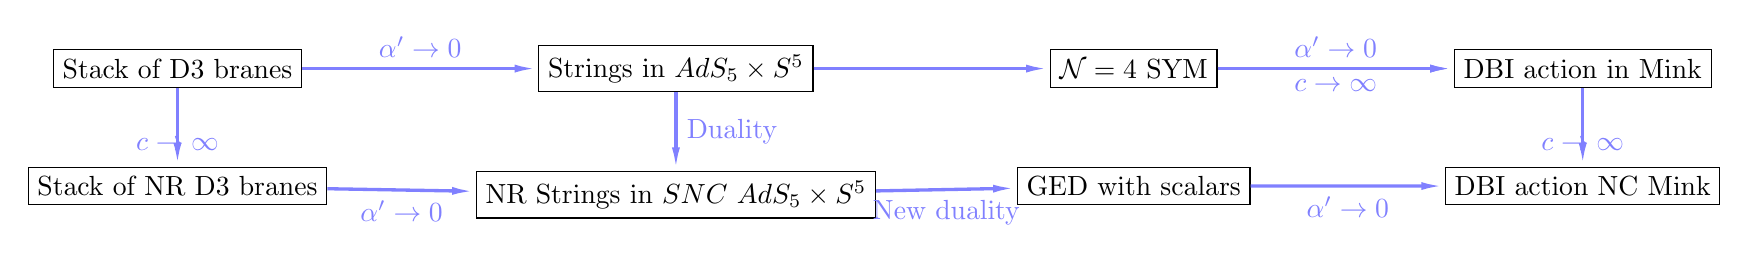
\begin{tikzpicture}[
    node distance=1cm and 3cm,
    arrow style/.style={blue!50, very thick, -{Latex[length=3mm, width=1mm]}}
]

% Nodes
\node (d3) [draw] {Stack of D3 branes};
\node (str1) [draw, right=of d3] {Strings in $AdS_5 \times S^5$};
\node (4sym) [draw, right=of str1] {$\mathcal{N}=4$ SYM};
\node (dbi1) [draw, right=of 4sym] {DBI action in Mink};
\node (nrstr) [draw, below=of str1] {NR Strings in $SNC\ AdS_5 \times S^5$};
\node (ged) [draw, below=of 4sym] {GED with scalars};
\node (dbi2) [draw, below=of dbi1] {DBI action NC Mink};
\node (d3nr) [draw, below=of d3] {Stack of NR D3 branes};

% Edges
\draw[arrow style] (d3) -- node [above] {$\alpha'\to 0$} (str1);
\draw[arrow style] (str1) -- node [above] {} (4sym);
\draw[arrow style] (4sym) -- node [above] {$\alpha'\to 0$} (dbi1);
\draw[arrow style] (str1) -- node [right] {Duality} (nrstr);
\draw[arrow style] (nrstr) -- node [below] {New duality} (ged);
\draw[arrow style] (ged) -- node [below] {$\alpha'\to 0$} (dbi2);
\draw[arrow style] (d3) -- node [below] {$c\to \infty$} (d3nr);
\draw[arrow style] (d3nr) -- node [below] {$\alpha'\to 0$} (nrstr);
\draw[arrow style] (4sym) -- node [below] {$c\to \infty$} (dbi1);
\draw[arrow style] (dbi1) -- node [below] {$c\to \infty$} (dbi2);

\end{tikzpicture}

\end{document}